\section{SPICE simulation results and analysis}

In this section, the circuit simulation of the AM Communication method demonstrated in Section \ref{gnuradio_am} will be presented using Qucs-s. 

\subsection{Circuit analysis}

In this simulation, the complete circuit consists on an AM Transmitter Block, a Channel Block, and finally the Receiver block as well. The simulated circuit can be found in Figure \ref{fig:Qucs_fullcircuit}.

\begin{figure}[H]§
    \centering
    \includegraphics*[width=0.7\textwidth]{Images/Qucs_fullcircuit.png}
    \caption{AM Communication circuit}
    \label{fig:Qucs_fullcircuit}
\end{figure}

The Transmitter block is implemented using, first a Summing OpAmp configuration, followed by one ideal switch, representing one Ideal Mixer, commuted by the Local Oscillator, with a frequency of $100 kHz$, resulting in the modulation of the input signal. 

Then to ensure that only the Base Band frequencies and the fundamental frequency of the carrier signal remain in the transmitted signal, an active Band Pass filter is used, with a central frequency corresponding to the carrier fundamental frequency, in this case $100 kHz$. This filter was implemented using the Multiple-Feedback topology, resulting in the 4\textsuperscript{th} order Bessel filter presented in Figure \ref{fig:Qucs_BPcircuit}.

\begin{figure}[H]
    \centering
    \includegraphics*[width=0.7\textwidth]{Images/Qucs_BPcircuit.png}
    \caption{Band Pass filter circuit}
    \label{fig:Qucs_BPcircuit}
\end{figure}

The Bessel approximation was adopted to guarantee a constant group delay around the carrier frequency, avoiding signal distortion. Finally, the transmitted signal is amplified using a Power Amplifier, implemented using a Non-Inverter OpAmp circuit.

Following the Transmitter Block, the channel is simulated by attenuating the transmitted signal and adding noise to it. 

Lastly, the signal is received by the Receiver Block, beginning with the Low Noise Amplifier, in this case, a Non-Inverter OpAmp with unitary gain, resulting in a Buffer configuration, followed by the step-down mixer, another Ideal Switch with the same frequency as the one present in the Transmitter Block. 

At last, the signal passes through an active Low Pass Filter, isolating the baseband signal form the remaining images of the modulated signal created by the Mixer in the demodulation process. The Bessel active Low Pass Multiple-Feedback Filter can be seen in Figure \ref{fig:Qucs_LPcircuit}.

\begin{figure}[H]
    \centering
    \includegraphics*[width=0.7\textwidth]{Images/Qucs_LPcircuit.png}
    \caption{Low Pass filter circuit}
    \label{fig:Qucs_LPcircuit}
\end{figure}

The higher filter order, is a result of the proximity between the baseband and the carrier frequency, originating a small transition region between the passband and the stopband. 

\subsection{Results}

\subsubsection{Low Pass and Band Pass Filters}

To measure the performance of the implemented filters, the frequency response was simulated, resulting in the Bode gain, phase and group delay graphics of both filters. First, the frequency response of the Band Pass Filter is presented in Figure \ref{fig:Qucs_BPBode}

\begin{figure}[H]
    \centering

    \begin{subfigure}[b]{0.5\textwidth}
        \centering
        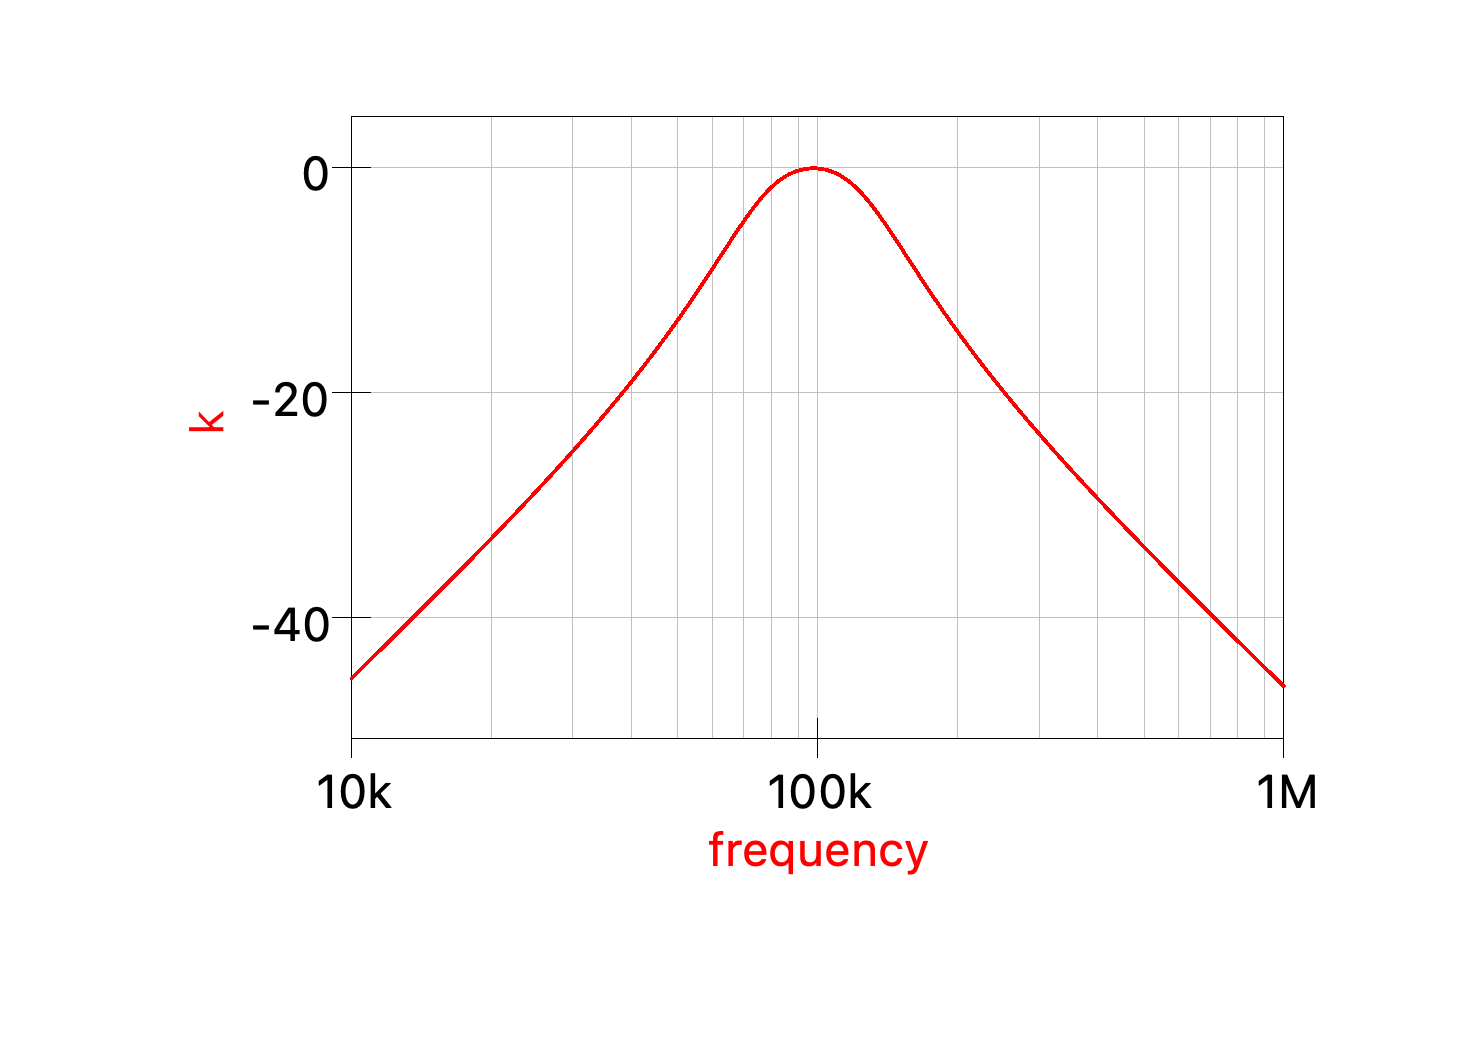
\includegraphics[width=\textwidth]{Images/Qucs_BPgain.png}
        \caption{Gain Bode Diagram.}
        \label{fig:Qucs_BPgain}
    \end{subfigure}%

    \begin{subfigure}[b]{0.5\textwidth}
        \centering
        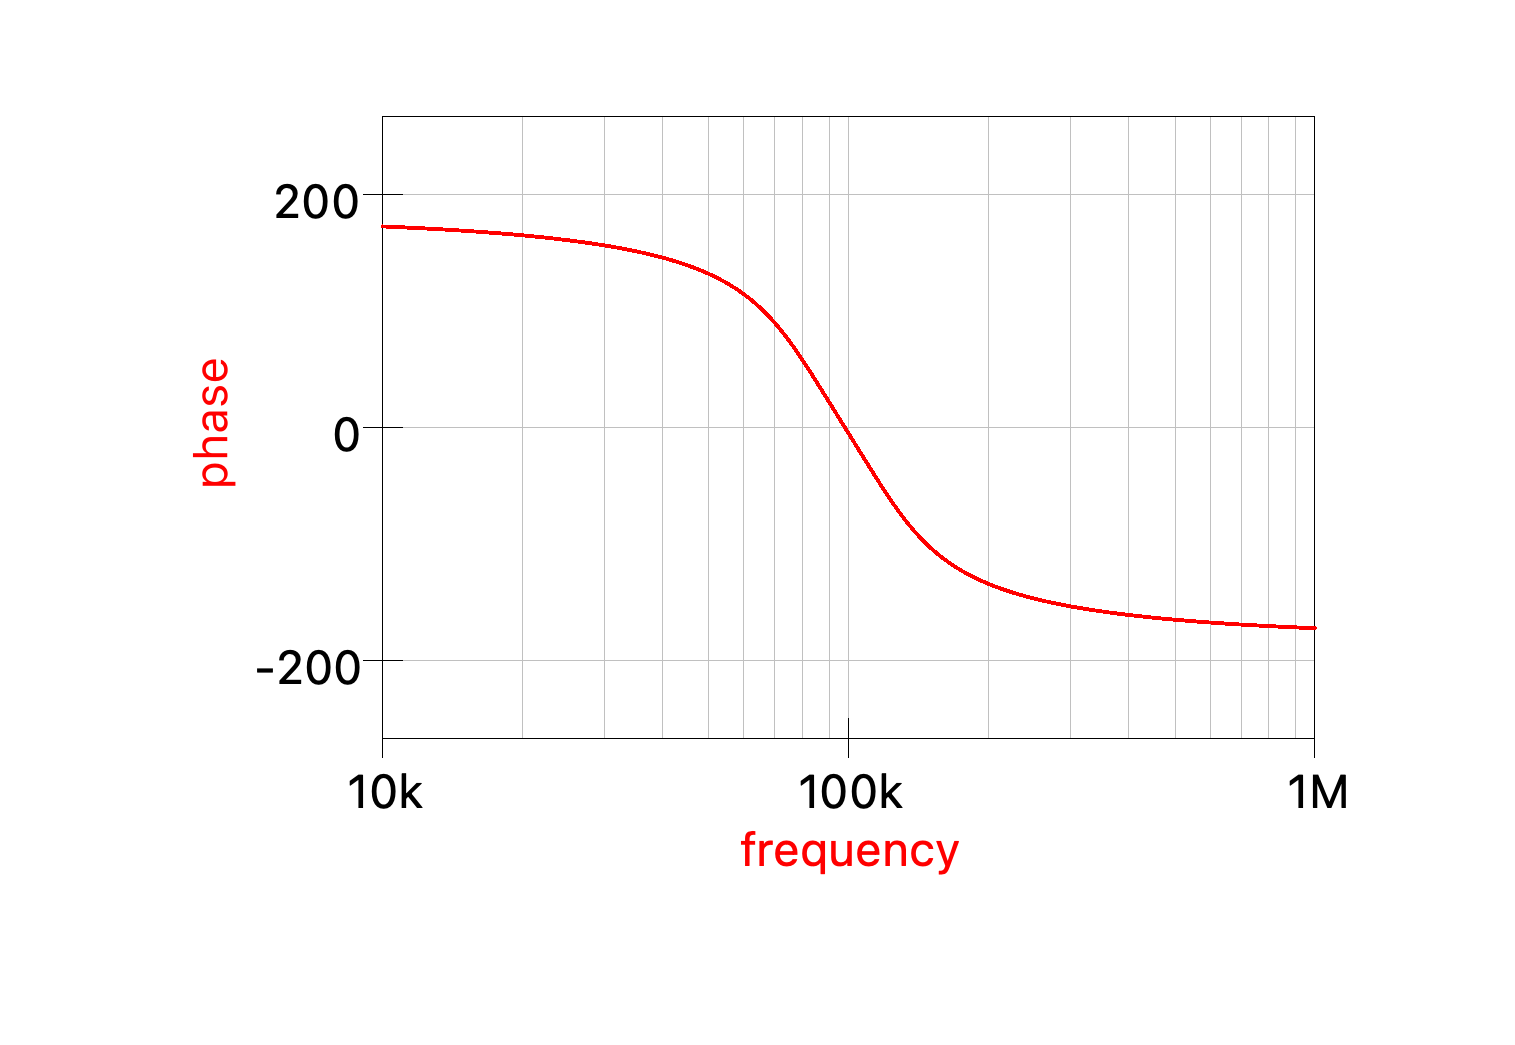
\includegraphics[width=\textwidth]{Images/Qucs_BPphase.png}
        \caption{Phase Bode Diagram.}
        \label{fig:Qucs_BPphase}
    \end{subfigure}%
    \begin{subfigure}[b]{0.5\textwidth}
        \centering
        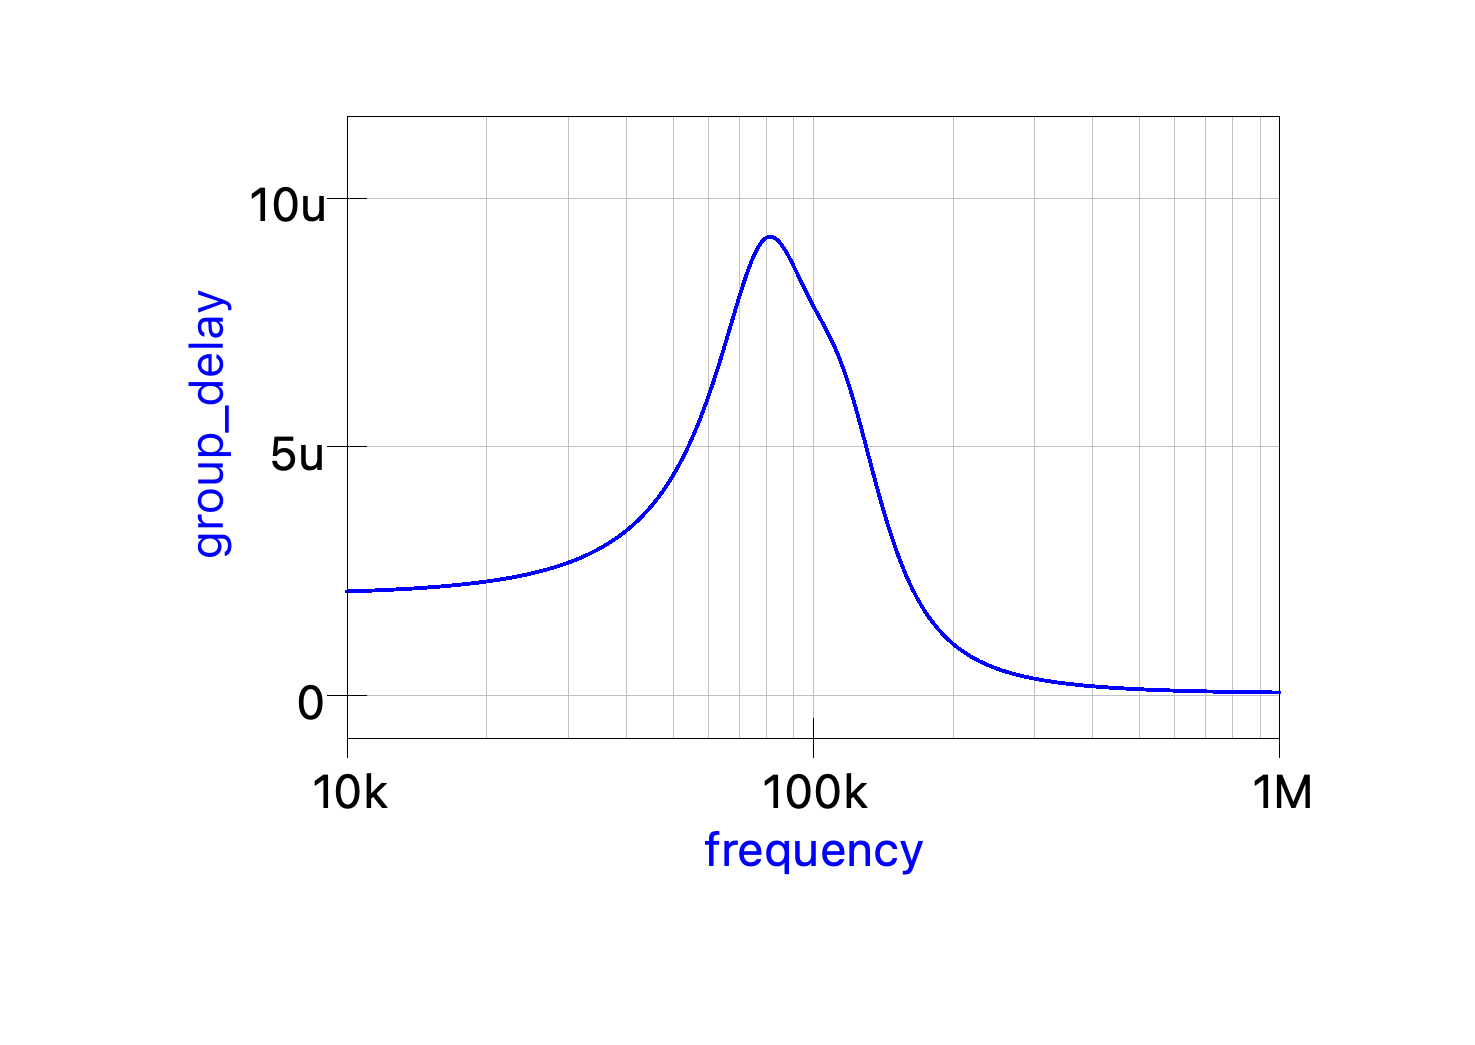
\includegraphics[width=\textwidth]{Images/Qucs_BPgd.png}
        \caption{Group Delay Bode Diagram.}
        \label{fig:Qucs_BPgd}
    \end{subfigure}

    \caption{Band Pass Filter Bode Diagrams}
    \label{fig:Qucs_BPBode}
\end{figure}

Analyzing the Bode Diagrams of the Band Pass Filter, it is possible to conclude that the baseband signal around the carrier frequency will not be affected by the filter, but all frequencies of the Local Oscillator signal excepted the fundamental will be eliminated, as pretended.

Passing to the Low Pass Filter, the frequency response of this filter is shown in Figure \ref{fig:Qucs_LPBode}

\begin{figure}[H]
    \centering

    \begin{subfigure}[b]{0.5\textwidth}
        \centering
        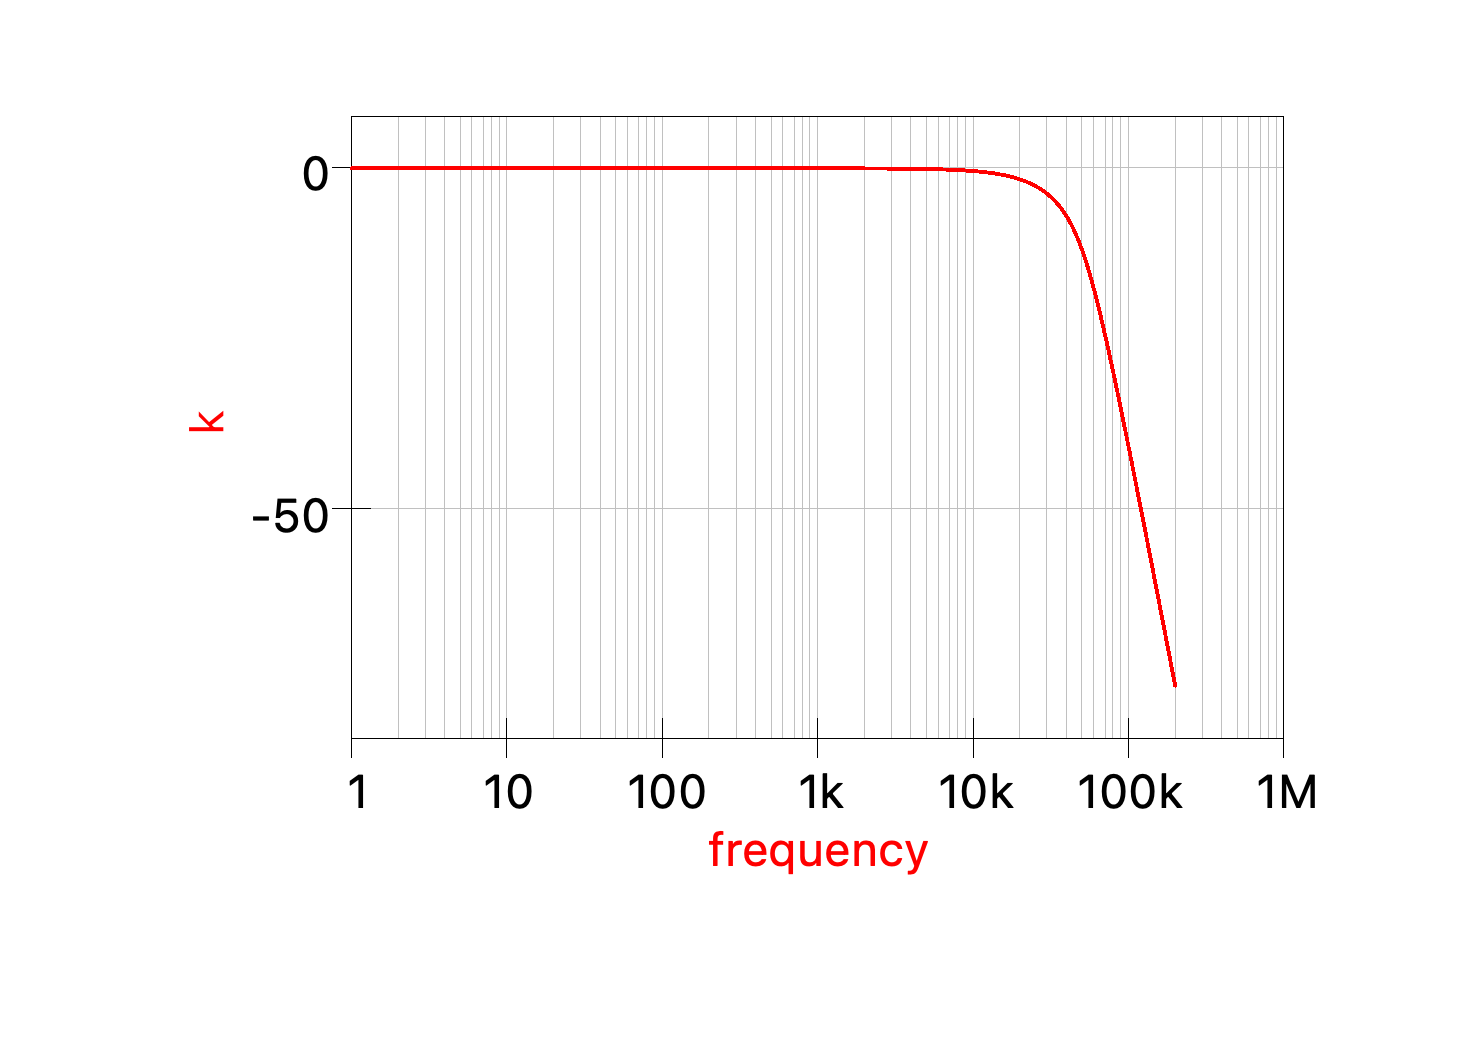
\includegraphics[width=\textwidth]{Images/Qucs_LPgain.png}
        \caption{Gain Bode Diagram.}
        \label{fig:Qucs_LPgain}
    \end{subfigure}%

    \begin{subfigure}[b]{0.5\textwidth}
        \centering
        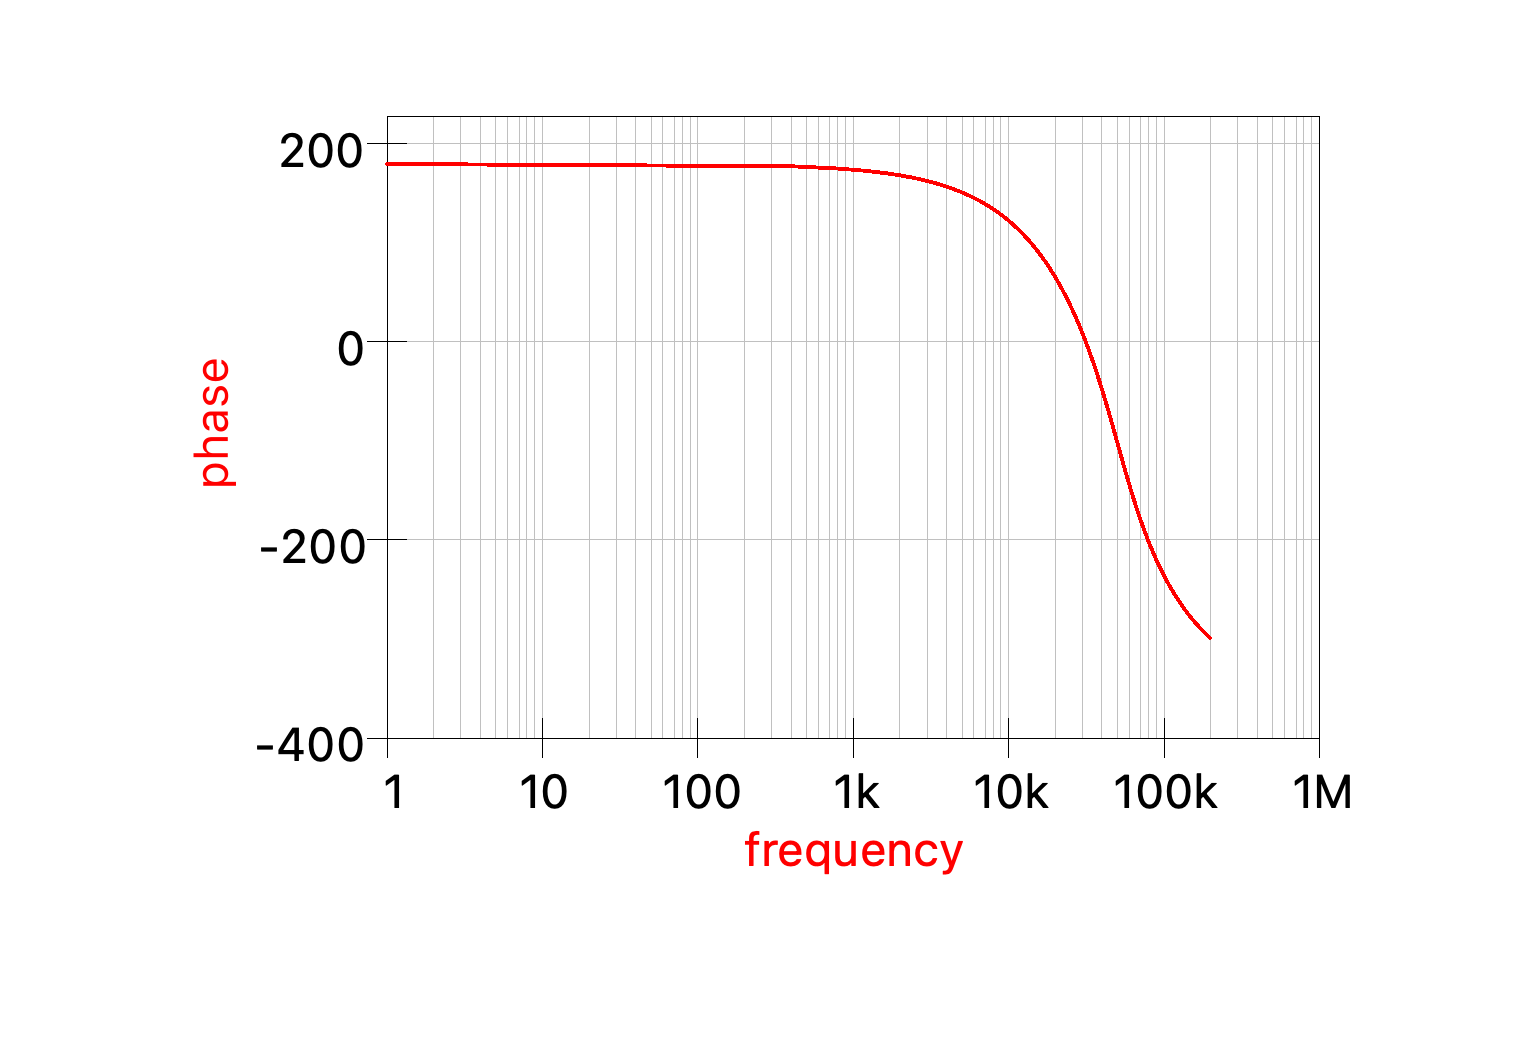
\includegraphics[width=\textwidth]{Images/Qucs_LPphase.png}
        \caption{Phase Bode Diagram.}
        \label{fig:Qucs_LPphase}
    \end{subfigure}%
    \begin{subfigure}[b]{0.5\textwidth}
        \centering
        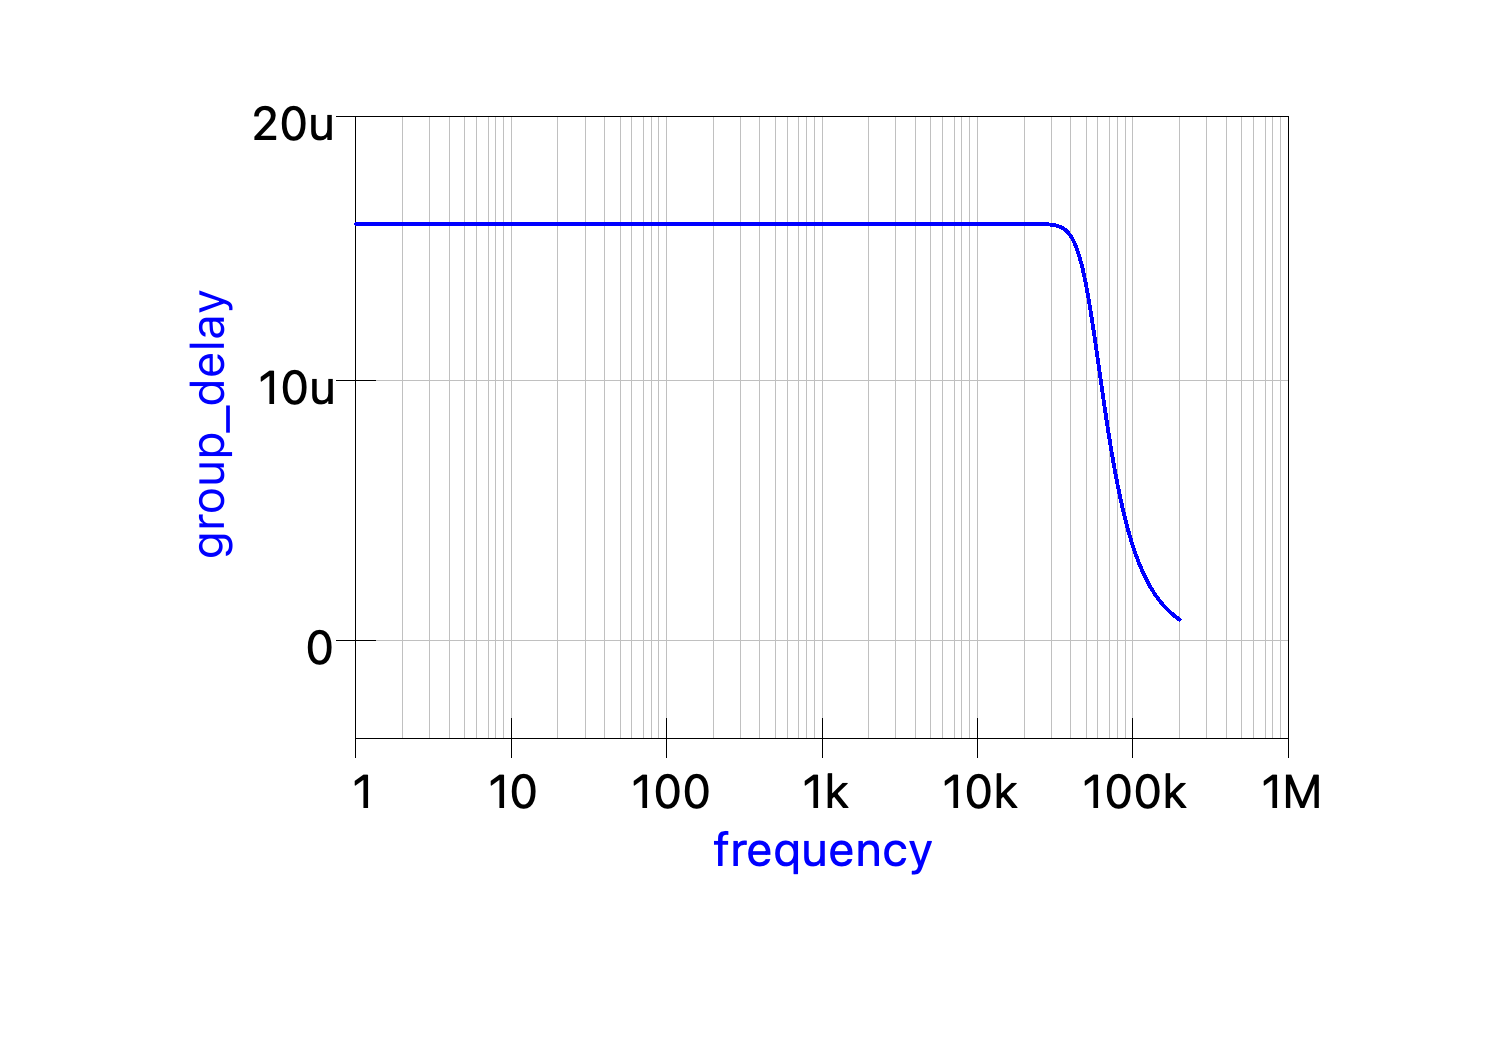
\includegraphics[width=\textwidth]{Images/Qucs_LPgd.png}
        \caption{Group Delay Bode Diagram.}
        \label{fig:Qucs_LPgd}
    \end{subfigure}

    \caption{Low Pass Filter Bode Diagrams}
    \label{fig:Qucs_LPBode}
\end{figure}

Looking at the Bode Diagrams of the Low Pass Filter, the gain diagram shows that for the baseband signal, there is no attenuation, but the same cannot be said for the carrier frequency, so, the output of the filter will only be the desired signal.

\subsubsection{Transmitter Block}

Since this circuit involves signals with different frequencies and amplitudes, the best way to analyze the results of each component is through the use of the Fourier Transformation, allowing the analysis of the effect of all parts of the circuit for each frequency. 

Starting with the mixer in the Transmitter, the Fourier Transform of the signal after the Mixer is shown in Figure \ref{fig:Qucs_vmod}

\begin{figure}[H]
    \centering
    \includegraphics*[width=0.7\textwidth]{Images/Qucs_vmod.png}
    \caption{Fourier Transform of the Mixer output}
    \label{fig:Qucs_vmod}
\end{figure}

In graphic above, is clear the presence of the carrier frequency and the baseband signal around and in its original location, so after the Band Pass Filter, the modulated signal is present in Figure \ref{fig:Qucs_vrf_fft}.

\begin{figure}[H]
    \centering
    \includegraphics*[width=0.7\textwidth]{Images/Qucs_vrf_fft.png}
    \caption{Fourier Transform of the Band Pass Filter output}
    \label{fig:Qucs_vrf_fft}
\end{figure}

Now only the desired band of frequencies is present in the signal. To confirm this fact, the signal in the time domain is displayed in Figure \ref{fig:Qucs_vrf}

\begin{figure}[H]
    \centering
    \includegraphics*[width=0.7\textwidth]{Images/Qucs_vrf.png}
    \caption{Band Pass Filter output}
    \label{fig:Qucs_vrf}
\end{figure}

Analyzing the signal in the time domain, it is possible to see the envelope and the carrier signal outlined by it. 

\subsubsection{Channel Block}

Now, to analyze the effect of the Channel Block, the signal after the Power Amplifier and at the Receiver can be compared, so both signal are presented in Figure \ref{fig:Qucs_vtx/vrx} in both time and frequency domains.

\begin{figure}[H]
    \centering
    \begin{subfigure}[t]{0.5\textwidth}
        \centering
        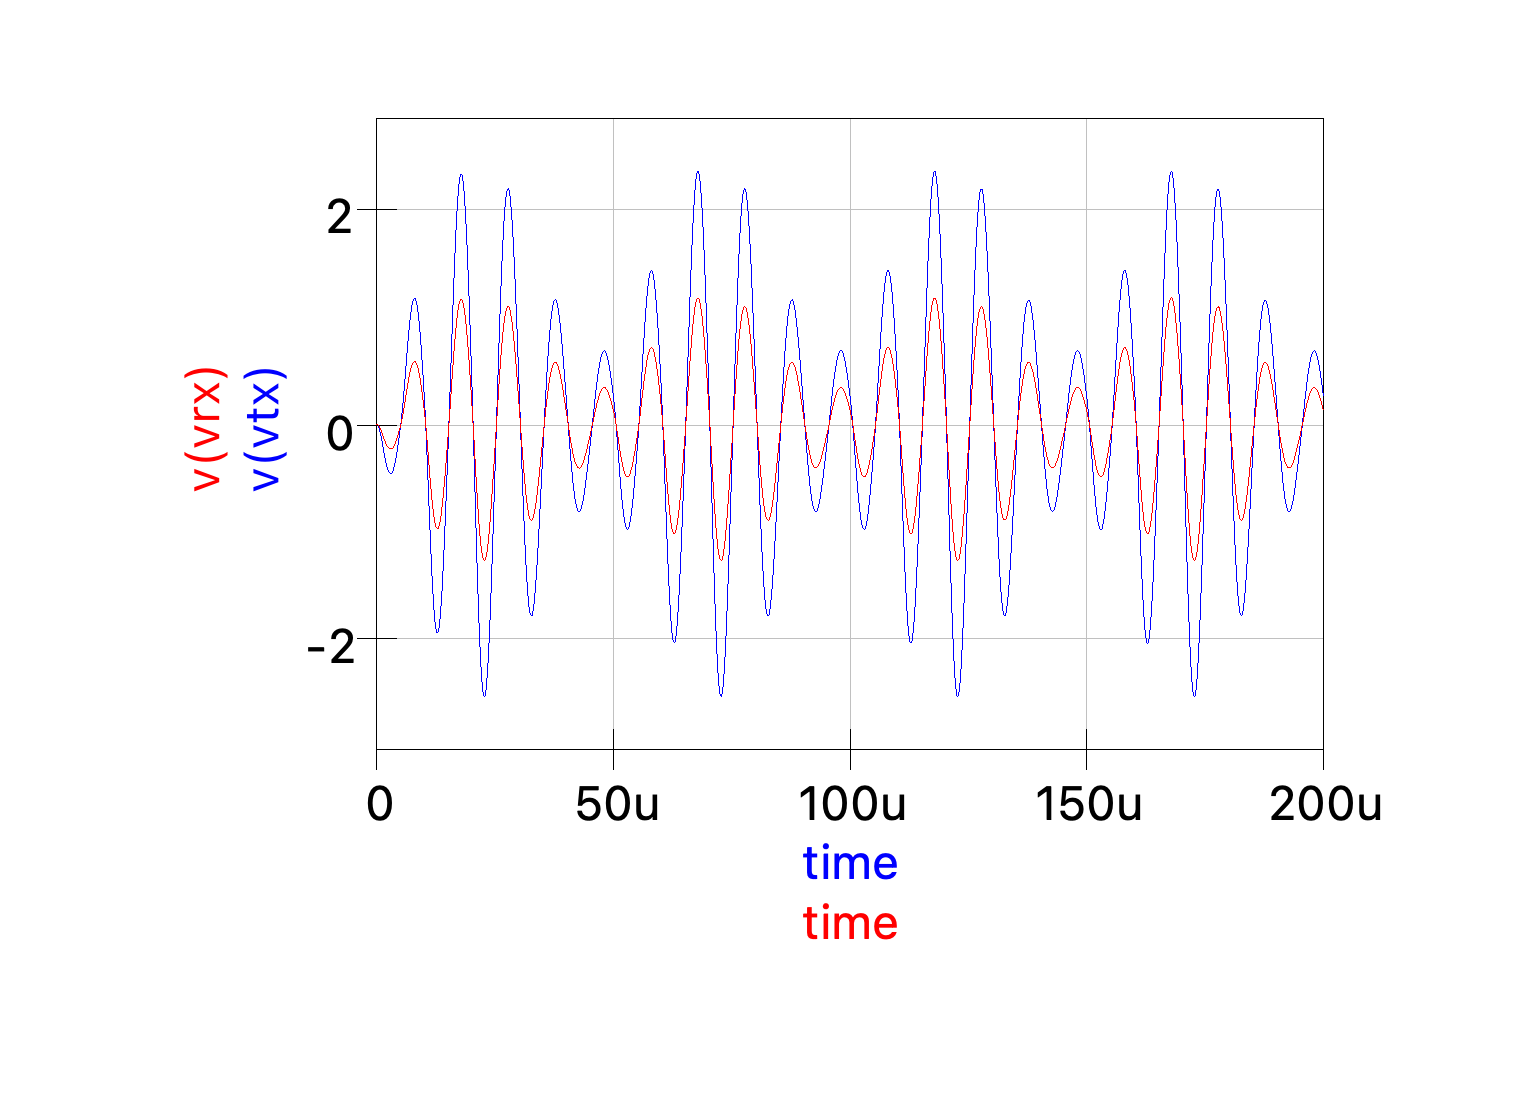
\includegraphics[width=\textwidth]{Images/Qucs_vtx:vrx.png}
        \caption{Time domain.}
        \label{fig:Qucs_vtx/vrx_time}
    \end{subfigure}%
    \begin{subfigure}[t]{0.5\textwidth}
        \centering
        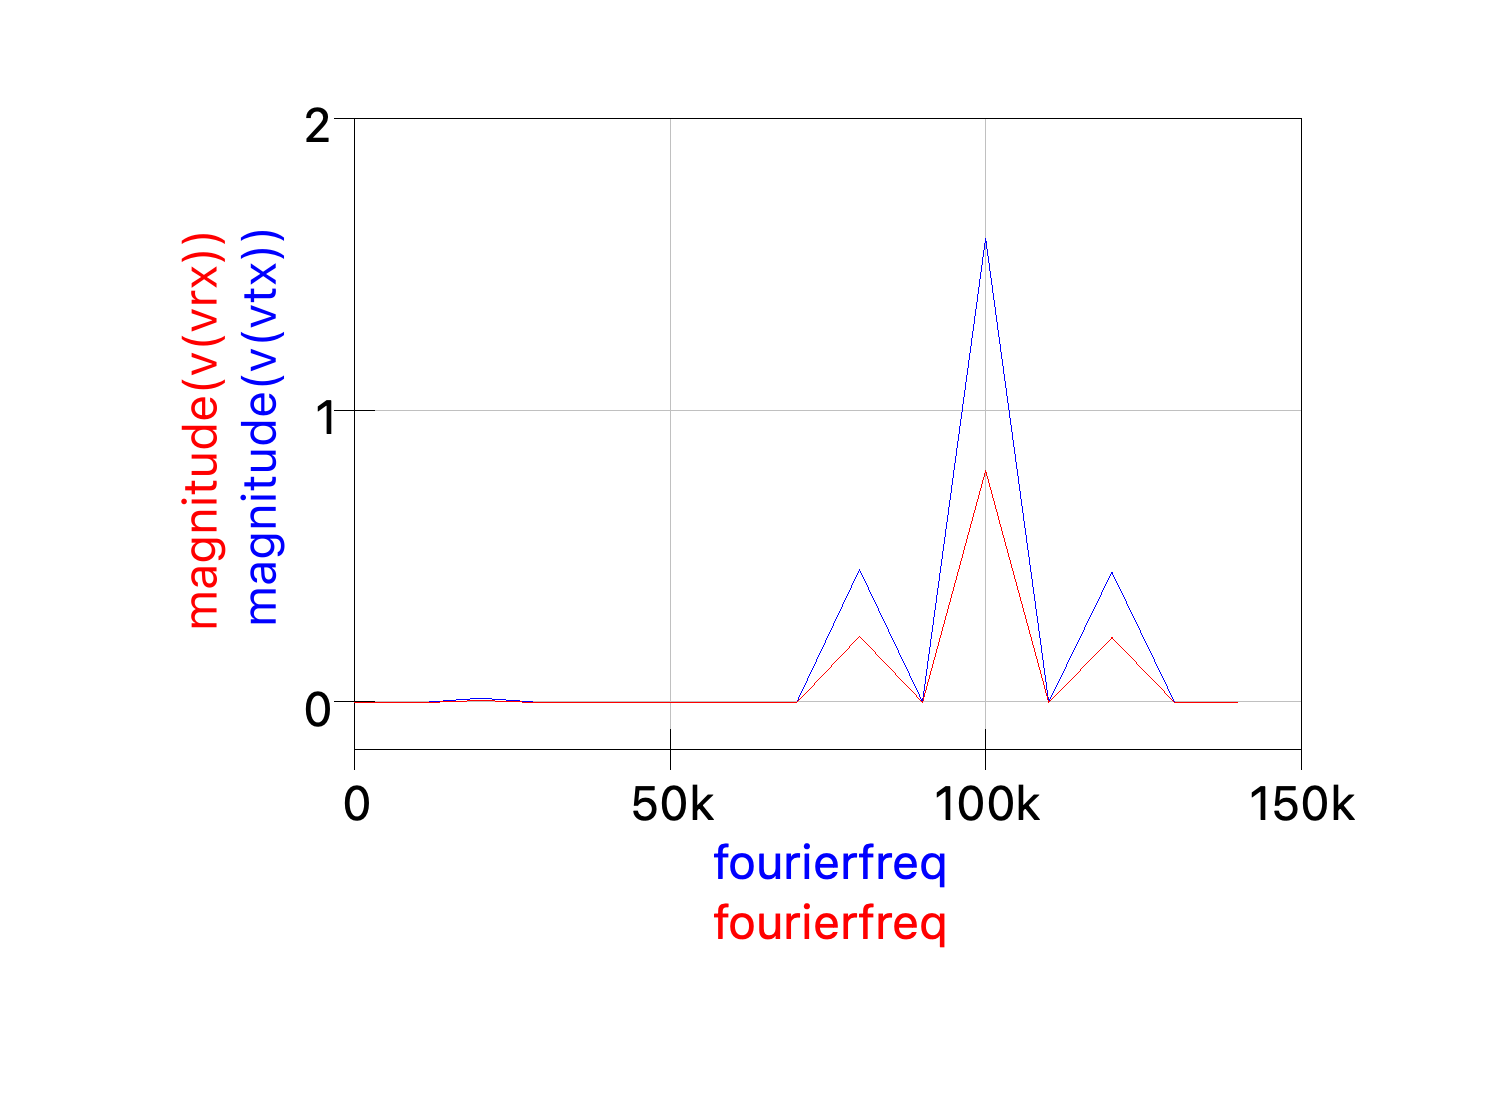
\includegraphics[width=\textwidth]{Images/Qucs_vtx:vrx_fft.png}
        \caption{Fourier Transform}
        \label{fig:Qucs_vtx/vrx_fft}
    \end{subfigure}
    \caption{Transmitted and received signals.}
    \label{fig:Qucs_vtx/vrx}
\end{figure}

Figure \ref{fig:Qucs_vtx/vrx} shows a difference in the amplitudes of both signals, validating the attenuation effect of the channel. 

\subsubsection{Receiver Block}

Passing then to the Receiver Block, the signal needs to be demodulated, so, after passing through the Mixer, the resulting signal's Fourier Transform is displayed in Figure \ref{fig:Qucs_vdemod}.

\begin{figure}[H]
    \centering
    \includegraphics*[width=0.7\textwidth]{Images/Qucs_vdemod.png}
    \caption{Fourier Transform of demodulated signal}
    \label{fig:Qucs_vdemod}
\end{figure}

After the mixer, the original signal is now in the original position, but the carrier frequency and the surrounding signal are still present, so, after the Low Pass Filter, the Fourier Transform of the filtered signal is shown in Figure \ref{fig:Qucs_vout}.

\begin{figure}[H]
    \centering
    \includegraphics*[width=0.7\textwidth]{Images/Qucs_vout.png}
    \caption{Fourier Transform of filtered received signal}
    \label{fig:Qucs_vout}
\end{figure}

Now, only the original baseband wave remains in the output, confirming the success of the AM Communication, to reinforce this observation, the comparison between the original transmitted signal and the one received can be seen in Figure \ref{fig:Qucs_vout/vin}.

\begin{figure}[H]
    \centering
    \includegraphics*[width=0.7\textwidth]{Images/Qucs_vin:vout.png}
    \caption{Transmitted and received signals}
    \label{fig:Qucs_vout/vin}
\end{figure}

Comparing both waves, it is clear that the signal integrity remains unchanged, only the amplitude suffered a reduction in its value. This reduction is the result of both mixer stages, the channel attenuation and also a slight reduction caused by the filters, since this were not ideal filters and with small order.